\documentclass[a4paper]{article}

\newcommand{\svcourse}{CST Part IA: Software Engineering and Security}
\newcommand{\svnumber}{1}
\newcommand{\svvenue}{Microsoft Teams}
\newcommand{\svdate}{2022-05-11}
\newcommand{\svtime}{15:00}
\newcommand{\svuploadkey}{CBd13xmL7PC1zqhNIoLdTiYUBnxZhzRAtJxv/ytRdM1r7qIfwMsxeVwM/pPcIo8l}

\newcommand{\svrname}{Dr Sam Ainsworth}
\newcommand{\jkfside}{oneside}
\newcommand{\jkfhanded}{yes}

\newcommand{\studentname}{Harry Langford}
\newcommand{\studentemail}{hjel2@cam.ac.uk}

% DO NOT add \usepackage commands here.  Place any custom commands
% into your SV work files.  Anything in the template directory is
% likely to be overwritten!

\usepackage{fancyhdr}

\usepackage{lastpage}       % ``n of m'' page numbering
\usepackage{lscape}         % Makes landscape easier

\usepackage{verbatim}       % Verbatim blocks
\usepackage{listings}       % Source code listings
\usepackage{graphicx}
\usepackage{float}
\usepackage{epsfig}         % Embed encapsulated postscript
\usepackage{array}          % Array environment
\usepackage{qrcode}         % QR codes
\usepackage{enumitem}       % Required by Tom Johnson's exam question header

\usepackage{hhline}         % Horizontal lines in tables
\usepackage{siunitx}        % Correct spacing of units
\usepackage{amsmath}        % American Mathematical Society
\usepackage{amssymb}        % Maths symbols
\usepackage{amsthm}         % Theorems

\usepackage{ifthen}         % Conditional processing in tex

\usepackage[top=3cm,
            bottom=3cm,
            inner=2cm,
            outer=5cm]{geometry}

% PDF metadata + URL formatting
\usepackage[
            pdfauthor={\studentname},
            pdftitle={\svcourse, SV \svnumber},
            pdfsubject={},
            pdfkeywords={9d2547b00aba40b58fa0378774f72ee6},
            pdfproducer={},
            pdfcreator={},
            hidelinks]{hyperref}

\renewcommand{\headrulewidth}{0.4pt}
\renewcommand{\footrulewidth}{0.4pt}
\fancyheadoffset[LO,LE,RO,RE]{0pt}
\fancyfootoffset[LO,LE,RO,RE]{0pt}
\pagestyle{fancy}
\fancyhead{}
\fancyhead[LO,RE]{{\bfseries \studentname}\\\studentemail}
\fancyhead[RO,LE]{{\bfseries \svcourse, SV~\svnumber}\\\svdate\ \svtime, \svvenue}
\fancyfoot{}
\fancyfoot[LO,RE]{For: \svrname}
\fancyfoot[RO,LE]{\today\hspace{1cm}\thepage\ / \pageref{LastPage}}
\fancyfoot[C]{\qrcode[height=0.8cm]{\svuploadkey}}
\setlength{\headheight}{22.55pt}


\ifthenelse{\equal{\jkfside}{oneside}}{

 \ifthenelse{\equal{\jkfhanded}{left}}{
  % 1. Left-handed marker, one-sided printing or e-marking, use oneside and...
  \evensidemargin=\oddsidemargin
  \oddsidemargin=73pt
  \setlength{\marginparwidth}{111pt}
  \setlength{\marginparsep}{-\marginparsep}
  \addtolength{\marginparsep}{-\textwidth}
  \addtolength{\marginparsep}{-\marginparwidth}
 }{
  % 2. Right-handed marker, one-sided printing or e-marking, use oneside.
  \setlength{\marginparwidth}{111pt}
 }

}{
 % 3. Alternating margins, two-sided printing, use twoside.
}


\setlength{\parindent}{0em}
\addtolength{\parskip}{1ex}

% Exam question headings, labels and sensible layout (courtesy of Tom Johnson)
\setlist{parsep=\parskip, listparindent=\parindent}
\newcommand{\examhead}[3]{\section{#1 Paper #2 Question #3}}
\newenvironment{examquestion}[3]{
\examhead{#1}{#2}{#3}\setlist[enumerate, 1]{label=(\alph*)}\setlist[enumerate, 2]{label=(\roman*)}
\marginpar{\href{https://www.cl.cam.ac.uk/teaching/exams/pastpapers/y#1p#2q#3.pdf}{\qrcode{https://www.cl.cam.ac.uk/teaching/exams/pastpapers/y#1p#2q#3.pdf}}}
\marginpar{\footnotesize \href{https://www.cl.cam.ac.uk/teaching/exams/pastpapers/y#1p#2q#3.pdf}{https://www.cl.cam.ac.uk/\\teaching/exams/pastpapers/\\y#1p#2q#3.pdf}}
}{}


\usepackage{float}
\usepackage{graphicx}

\begin{document}

\begin{examquestion}{2009}{3}{5}

\subsubsection*{In what ways should the information goods and services
sector be less or more severely affected by the credit crunch than the rest
of the economy?}

\section*{The Essay}

\subsection*{Introduction}

The global financial crisis plunged most of the worlds developed economies
into a deep recession, the effects of which we are still experiencing today.
Over-optimism in economic outlook led bankers to lend excessively with
minimal capital underpinning the loans. This meant that banks had the
potential to make a lot of money but were particularly vulnerable to market
volatility. Many of the loans made were subprime -- to people who had
poor histories and low likelihoods of full repayment. Due to the lessons
learnt and the instability of the financial institutions, loans became far
sparser causing a ``credit crunch''.

The information goods and services sector initially appears likely to become a
victim of the crisis; investments in information goods and services are
characterised as high-risk-high-reward due to the strong networking effects
observed in the industry. However, many companies offering information goods
and services have high lock-in; which means the easiest way for clients to
save money (which is what they will want to do during a recession) is to
stay with the company.

\subsection*{More affected}

Loan availability for companies in the information goods and services sector
will decrease dramatically -- especially for smaller companies without a
proven track record. Due to the dot-com bubble bursting (the economic crisis
before the global financial crisis), investments in web companies (which
make up an ever-increasing portion of the information goods and services
sector) have been perceived as risky. Established websites may find funding,
however it's likely that many small online businesses will be unable to
find the necessary funding. This is likely to lead to a decrease in the
growth of the internet.

The customers of information goods and services align with the demographic
who are most severely affected by the credit crunch. Many information goods
are targeted at affluent customers: office workers, people who can afford an
internet connection and people who have good TVs. This demographic is also
the demographic who were most severely affected by the credit crunch --
taking out loans to buy new properties. Studies in the US indicated that
people who had money were affected the most by the credit crunch -- people who
didn't have money didn't have the money to lose. Although the numerical
decrease in assets was comparatively low, in recessions people prefer to
have a higher amount of liquid assets. This means people spend less money as
they try to accumulate enough money for them to feel safe in the new
economic climate. Many people who have money to spend (people who use
information goods and services) are therefore likely to try to save money,
leaving companies in the information goods and services sector with less
revenue.

Furthermore, a higher proportion of companies in the information goods and
services sector follow the ``startup'' model -- where a business with no
record gets a large investment and turns losses for several years before
establishing itself and turning a profit several years after it begins
trading. This business model requires loans and hence lenders who are happy
to take a risk. However, lenders are unlikely to be as willing to loan money
in the future and therefore this business model will become inviable. Since
information goods and services have a higher proportion of companies
following this model.

Due to strong network effects, the information goods and services sector is
particularly prone to monopolisation. This will be exacerbated by the credit
crunch. To break monopolies, new businesses need to form and grow. However,
with a lack of availability of loans this will not be possible to the extent
required to break monopolies. Therefore, monopolies in the information goods
and services sector (such as Facebook, Google and Amazon) will remain
largely unchallenged for years. This will result in an even more monopolised
industry. The result of this is that the market could be manipulated, making
the monopolies significant amounts of money but damaging the sector as a whole.

The information goods and services sector thrives off two types of product:
new products and optimisations. New products are often high-risk investments
with possible high yields -- in a recession investors will try to invest
where they are likely to have guaranteed gains rather than risky investments.
Therefore this side of the information goods and services sector is likely
to be neglected. The other type of product which companies in the
information goods and services sector sell are optimisations -- outside of a
recession, companies are looking for optimisations to increase efficiency,
in the long-run. However, during a credit crunch many companies will not
have sufficient funding to afford these optimisations. Although cost-saving
optimisations are exactly what the information goods and services sector can
offer, almost no company will be willing to spend the money required to save
money. Therefore demand for all types of product offered by the information
goods and services sector will decrease. This will cause the industry to
experience slow growth. Historically, technology companies have experienced
very high growth -- this has encouraged investors. Flatlining growth in a
risky sector is likely to discourage investors in the future -- who may view
even safe companies in the sector as subprime, preventing new
companies challenging monopolies for many years.

Regrettably, many information goods can be pirated. While most people will
not pirate material, if economic pressure becomes severe enough it is likely
to increase the number of people who pirate content. Currently, almost 20\% of
all information material consumed is pirated. It's becoming increasingly
harder to manage pirated material due to the size of the internet and
popularity of peer-to-peer networks. A dramatic rise in piracy rates due to
economic pressure may cripple the information goods and services sector.

Creating information goods or services: books, songs and software is
expensive and time-consuming. Without sufficient investment from loans,
companies and the industry may not be able to create new information. This
could potentially result in a lull where there is no promising information
being created and investors become underwhelmed.

\subsection*{Less Affected}

Many information goods and services companies benefit from a very high
lock-in. This means that it is often hard for companies and clients to
switch to other companies (or stop using the product altogether). Therefore,
companies who do not go bankrupt as a result of the credit crunch will find
that the cheapest way for them to continue trading is to continue using their
current service providers. This means that information service providers are
unlikely to observe a significant decrease in income or observe significant
moves away and therefore the income of established companies could be largely
unaffected.

Many companies in the sector have very low marginal costs and low fixed
costs. Most of the cost of running a company in the information goods and
services sector comes from the cost of creating new products -- consider
Google, where the majority of its expenditure comes from the creation of new
services rather than the maintenance of existing services. Therefore, many
information companies expenses are ``optional'' -- they can choose not to
create new products for a short period of time if required. Therefore it is
very hard to make an information company bankrupt -- if they face financial
concerns they can idle for several months or focus their efforts only on
the most promising projects until the outlook looks better.

The information goods and services sector is one of the most exciting
sectors -- there are consistently new services and inventions and
``must-see'' material. This excitement may make it somewhat resilient to the
crisis -- investors could expect the sector to perform well in the long-run
or may simply like the companies and the products too much. This could
counteract the effect of the credit crunch and result in good funding and
challengers to the monopolists.

\subsection*{Conclusion}

The credit crunch is the most significant financial event since the great
depression and the effects of it will reverberate through the economy for
years. The information goods and services sector is likely to be highly
affected: it will be reshaped and monopolised, face slow growth and be
undervalued for years to come -- but is unlikely to face widespread bankruptcy.

\end{examquestion}

\begin{examquestion}{2020}{7}{3}

\begin{enumerate}[label=(\alph*)]

\item Define the following terms, providing examples to illustrate their
meaning.

\begin{enumerate}[label=(\roman*)]

\item Pareto improvement

A pareto improvement is a change which leaves one party better off but does
not leave any other party worse-off.

Consider two allocations: player 1 gets 0 and player 2 gets 0; or player 1
gets 0 and player 2 gets 1. The second allocation is a pareto improvement on
the first allocation as player 2 benefits at no cost to player 1.

\item Pareto efficient allocation

A pareto efficient allocation is an allocation such that there is no pareto
improvement.

An example of this would be an allocation of funds where one
player gets everything. No other player can get anything without it coming
from the first player and therefore the allocation is pareto efficient.

\item Utility

Utility is the value that a consumer places on a good.

Utility is usually non-linear in number of goods. For example here is a
graph of utility against number of free meals per day. The utility for a
small number of free meals per day is high, but tapers off quickly.

\begin{figure}[H]
\centering
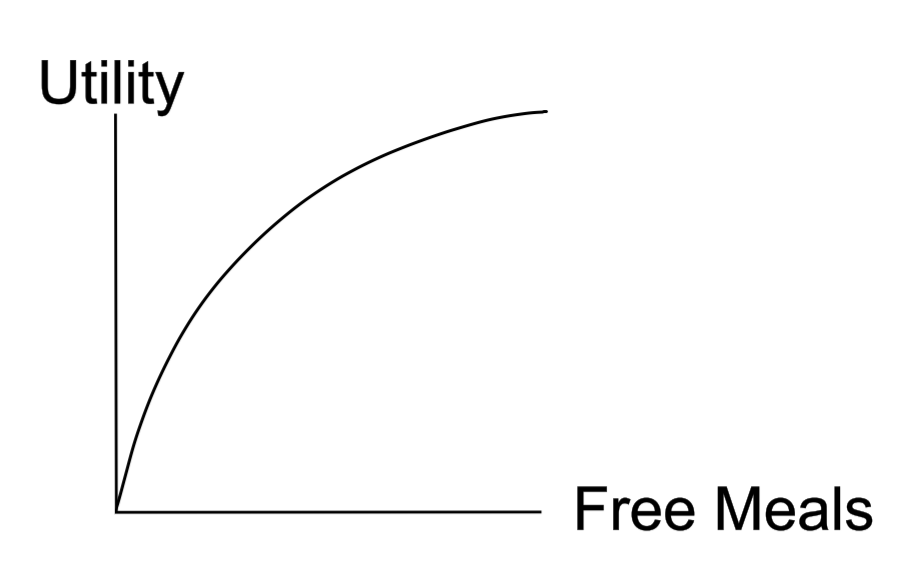
\includegraphics[width=0.5\textwidth]{./utility}
\end{figure}

\end{enumerate}

\item Explain the theorems of welfare economics, comparing and contrasting
classical utilitarian welfare and Rawlsian welfare.

\begin{itemize}

\item The first theorem of welfare economics states that market equilibrium
is a pareto efficient allocation.

If a market is in equilibrium then the allocation is not pareto efficient --
else some company will change the structure such that they benefit without
damaging any other company. Essentially, if we view the market as a
$n$-dimensional graph then the equilibrium is a local maxima.

\item The second theorem of welfare economics states that any pareto efficient
allocation can be reached by market forces if preferences are convex.

There is some initial set of endowments such that locally optimal decisions
by companies will lead to any pareto efficient allocation. Essentially, if
we view the market as an $n$-dimensional function then there is some point
such that gradient descent will reach any local minima.

\item Classical utilitarian welfare views welfare as the total utility across
the whole population. This is the approach taken by most countries -- to
maximise GDP .

\item Rawlsian welfare maximises the minimum utility -- the welfare of the
state is the utility of the poorest person. This approach is that of a
compassionate society and is taken by only the most liberal countries.

\end{itemize}

\item Do you expect the free market to solve the privacy problem?

Many technology companies are encouraged to gather as much data on customers
as possible to maximise their revenue. Whether this is Google gathering data
to help place advert slots from ad auctions or Amazon gathering data to
assess which products to recommend to us or Spotify collecting data to
recommend new songs; almost all major companies are heavily incentivised to
collect as much data as possible. Gathering as much data as is legal is
pareto optimal -- the more data companies gather, the more data they can use
and the better personalisation they can offer.

Most consumers follow defaults -- there is simply not enough publicity about
the data that companies collect and users don't care enough. Users
will accept cookies or terms of service which release their private
data without reading them. Companies do offer services without
``personalisation'' -- you can disable tailored adverts on almost any
platform and remove access for data; most companies benefit more from a
user with data collection settings disabled than no user and therefore offer
such settings. Most users simply don't bother enabling these settings.

As mentioned earlier, gathering as much data as is legal is pareto efficient
. For the free-market to solve the privacy problem, this would have to
change. This can happen by either decreasing the amount of data which is
legal to gather or by a societal shift. Changing the law is not performed by
free market forces, however a societal shift could be. If a large company
were to have a data scandal then other large companies could come under
public scrutiny. It may then become societally unacceptable to have invasive
privacy policies. If having such a privacy policy were to cause people to
leave services then it would be a pareto improvement for large companies to
have a more respectful privacy policy. However, this is unlikely to apply to
smaller companies and websites -- who do not have reputations to protect.

I think it is unlikely for free-market forces to solve the privacy
problem -- it's not currently pareto optimal and for it to become pareto
optimal would require a full societal shift, which seems unlikely.

\end{enumerate}

\end{examquestion}

\begin{examquestion}{2010}{4}{8}

\begin{enumerate}[label=(\alph*)]

\item In a hawk-dove game, doves share food, hawks take food from doves and
hawks fight each other (with a certain risk of death).

\begin{enumerate}[label=(\roman*)]

\item Write out this game in strategic form.

Encounters happen when two birds find food of value $v$. If two doves find
food then they will share it, so they both get $\frac{v}{2}$. If a dove and
a hawk finds food then the hawk steals from the dove -- the hawk gets $v$
and the dove gets $0$. If two hawks find food then they will fight for it;
fighting has total cost $c$ and therefore the gain to each hawk is $\frac{v - c
}{2}$ which can be negative.

\begin{table}[H]
\centering
\begin{tabular}{c|c c}
& Hawk & Dove \\
\hline
Hawk & $\left( \frac{v - c}{2}, \frac{v - c}{2} \right)$ & $(v, 0)$ \\
Dove & $(0, v)$ & $\left( \frac{v}{2}, \frac{v}{2} \right)$
\end{tabular}
\end{table}

\item Under what circumstances will there be an equilibrium with non-zero
numbers of hawks and doves?

There is an equilibrium with a non-zero number of doves and hawks when $c >
v$.

If $c < v$ then the nash equilibrium is that all birds are hawks -- if
the other bird is a dove then it is beneficial to be a hawk; and if the
other bird is a hawk then it is beneficial to be a hawk (as
$\frac{v - c}{2} > 0$ so in an encounter with a hawk you get more if you're
a hawk).

If $c = v$ then all birds are hawks and they all starve as the same logic as
above holds.

\item What will this equilibrium be? Justify your answer.

With $p$ as the proportion of birds which are hawks; the equilibrium is:
\[
p = \frac{v}{c}
\]

If the expected return from being a hawk was greater than the expected
return from being a dove, then the game is not in equilibrium -- as the
number of hawks will be increasing. An analogous argument holds for doves.
Therefore, we can conclude that the equilibrium occurs when the expected
return from being a hawk is equal to the expected return from being a dove.

We can form an equation from this and solve:

\[
\begin{split}
\mathbb{E}(d)
&= \mathbb{E}(h) \\
p\cdot 0 + (1 - p) \cdot \frac{v}{2}
&= p \cdot \left( \frac{v - c}{2} \right) + (1 - p) \cdot v \\
p \cdot c &= p\cdot v - v + p \cdot v + 2 \cdot v - 2 \cdot p \cdot v \\
p \cdot c &= v \\
p &= \frac{v}{c} \\
\end{split}
\]

As required, therefore the proportion of birds which are hawks in a
dove-hawk game $p$ where $c > v$ will be $\frac{v}{c}$.

\end{enumerate}

\item Why might people be more aggressive online than they are in
face-to-face encounters?

The cost of encountering another aggressive person online is significantly
less than the cost of encountering another aggressive person in a
face-to-face encounter and therefore the equilibrium has a higher proportion
fo aggressive people.

We can model human interactions as a dove-hawk game.

In-person encounters have a high cost -- if an aggressive person encounters
another aggressive person then they get in a fight and get injured or go
to jail. This is substantially more than the benefit from being nasty to
someone who is nice -- the \pounds 100 they have in their wallet.

The cost of encountering another aggressive person online is substantially
less. The worst that happens is an argument and blocking the other person.
In many cases this is almost zero cost and therefore under the dove-hawk
logic, there is no incentive to be nice.

\end{enumerate}

\end{examquestion}


\end{document}